\documentclass[conference]{IEEEtran}
\IEEEoverridecommandlockouts
\usepackage{cite}
\usepackage{amsmath,amssymb,amsfonts}
\usepackage{algorithmic}
\usepackage{graphicx}
\usepackage{textcomp}
\usepackage{booktabs}
\usepackage[hidelinks]{hyperref}
\usepackage{tabularx}
\usepackage{tikz}
\usetikzlibrary{shapes.geometric, arrows, positioning, fit, calc}

\def\BibTeX{{\rm B\kern-.05em{\sc i\kern-.025em b}\kern-.08em
    T\kern-.1667em\lower.7ex\hbox{E}\kern-.125emX}}

% Force IEEE to use "Keywords"
\renewcommand\IEEEkeywordsname{Keywords}

\begin{document}

\title{Development of an Edge AI Pest Monitoring and Soil-Gated Control System for Cavendish Banana (\textit{Musa acuminata}) Plantations}

\author{\IEEEauthorblockN{Lemuel Blaya\textsuperscript{1}}
\IEEEauthorblockA{\textit{Electronics Engineering Program} \\
\textit{College of Engineering Education}\\
\textit{University of Mindanao}\\
Matina, Davao City, Philippines \\
l.blaya.551860@umindanao.edu.ph \\
{\scriptsize ORCID: 0009-0008-6562-9201}}
\and
\IEEEauthorblockN{Angelo Diaz\textsuperscript{1}}
\IEEEauthorblockA{\textit{Electronics Engineering Program} \\
\textit{College of Engineering Education}\\
\textit{University of Mindanao}\\
Matina, Davao City, Philippines \\
a.diaz.552518@umindanao.edu.ph \\
{\scriptsize ORCID: 0009-0002-2311-6412}}
\and
\IEEEauthorblockN{Blessie Angelie Mugat\textsuperscript{1}}
\IEEEauthorblockA{\textit{Electronics Engineering Program} \\
\textit{College of Engineering Education}\\
\textit{University of Mindanao}\\
Matina, Davao City, Philippines \\
b.mugat.560558@umindanao.edu.ph \\
{\scriptsize ORCID: 0009-0009-1803-689X}}
}

\maketitle

\thispagestyle{plain}
\pagestyle{plain}

\begin{abstract}
Cavendish banana plantations in the Davao Region experience significant yield losses from insect pests, leading to environmentally degrading calendar-based pesticide spraying. The general objective of this study is to develop a fixed-post Internet of Things (IoT) prototype utilizing an ESP32-C6 and a lightweight Convolutional Neural Network (CNN) to autonomously identify pests and execute a soil-gated spray actuation. Guided by explicit hypotheses of detection equivalence and actuation reliability, system feasibility and detection accuracy will be evaluated via a servo-driven controlled bench validation and an outdoor potted-plant simulation. Using a Two One-Sided Tests (TOST) procedure, the prototype is designed to establish empirical equivalence in detection accuracy against ground-truth benchmarks while verifying a minimum 7-day battery autonomy under monsoon conditions. Ultimately, this hardware validation lays the required engineering groundwork for scalable and sustainable precision agriculture frameworks.
\end{abstract}

\vspace{1em}

\begin{IEEEkeywords}
Edge Computing, TinyML, LoRaWAN, Precision Agriculture, Transfer Learning
\end{IEEEkeywords}

\section{Introduction}
Pest infestations in Cavendish banana (\textit{Musa acuminata}) plantations pose a continuous threat to agricultural stability in the Davao Region, where local pests such as \textit{Thrips hawaiiensis} \cite{reyes2022} and \textit{Fusarium} wilt vectors \cite{nozawa2023} endanger crop viability. Furthermore, these pests utilize surrounding agricultural weeds as alternative hosts, compounding the difficulty of eradication \cite{vercellino2022}. Conventional pest management relies heavily on blanket pesticide application; however, this calendar-based spraying degrades soil microbial communities and enzyme activities \cite{liu2020} while introducing chemical toxicity risks.

The integration of the Internet of Things (IoT) in agriculture has provided viable solutions for precision resource management \cite{zeyliger2023}. Recent implementations demonstrate that intelligent pest management can be achieved using edge sensors \cite{ahmed2024}, and computer vision (CV) integrated with IoT can monitor insect networks autonomously \cite{cardoso2022}. Secure data transfer protocols further ensure that these distributed sensing networks can reliably deliver field metrics to cloud-based decision systems \cite{deoliveira2025}.

In resource-constrained environments, continuous deployments confirm that lightweight Convolutional Neural Network (CNN) architectures can achieve high counting accuracy for agricultural targets \cite{bereciartua2023}. To optimize processing on edge hardware, recent frameworks employ transfer learning \cite{hayajneh2023}, demonstrating that fine-tuning pre-trained models on microcontrollers like the ESP32 meets strict agricultural inference requirements without the need for massive datasets \cite{donskoy2025}. Techniques such as image segmentation \cite{singh2022}, Region of Interest (ROI) frame-differencing \cite{prasetyo2022}, and localized leaf disease segmentation \cite{chaudhari2023} are also utilized to minimize computational overhead before classification.

Despite these advancements, a critical gap remains between edge-based data acquisition and autonomous physical actuation. Existing systems frequently operate as isolated monitoring tools \cite{wang2024} or generic disease classifiers \cite{sneineh2023}. Unlike previous approaches that simply log pest presence, there is a distinct need for a localized system that bridges monitoring and actuation by integrating automated control logic strictly constrained by abiotic environmental safety parameters, such as soil saturation, to prevent chemical runoff.

\subsection{Objectives of the Study}
The general objective of this study is to develop and evaluate a fixed-post edge AI pest monitoring and actuation prototype. The specific objectives are listed in decreasing order of contribution, with each anchored to the two-semester capstone timeline:
\begin{enumerate}
    \item To develop, within Semester 1, a TinyML CNN utilizing transfer learning on a MobileNetV2 backbone that attains a mean $F1$-score of $\geq 85\%$ on a held-out test set, trained with a negative class dataset to reject environmental noise;
    \item To empirically determine, during the Phase 1 bench validation in Semester 1, the accuracy and reliability of the actuation logic, establishing statistical equivalence between prototype pest counts and ground-truth counts (TOST, $\alpha = 0.05$);
    \item To execute, during the Phase 2 potted-plant test in Semester 2, an automated control protocol anchored to derived Economic Injury Level (EIL) parameters, achieving a soil-gated actuation reliability of $\geq 95\%$ with a false-spray rate of $\leq 5\%$; and
    \item To validate, during Semester 2, a minimum 7-day battery autonomy under continuous worst-case monsoon conditions.
\end{enumerate}

\subsection{Research Hypotheses}
Consistent with the developmental-experimental design, the study tests the following hypotheses at $\alpha = 0.05$:
\begin{itemize}
    \item \textbf{$H_{0,1}$ (Detection):} The prototype's CNN-derived pest counts are \emph{not} statistically equivalent to the ground-truth mechanical counts within the pre-specified equivalence margin $\pm\delta$.
    \item \textbf{$H_{a,1}$ (Detection):} The prototype's CNN-derived pest counts \emph{are} statistically equivalent to the ground-truth counts within $\pm\delta$ (evaluated via TOST).
    \item \textbf{$H_{0,2}$ (Actuation):} The soil-gated actuation reliability does not differ from the $\geq 95\%$ target criterion.
    \item \textbf{$H_{a,2}$ (Actuation):} The soil-gated actuation reliability meets or exceeds the $95\%$ target criterion.
    \item \textbf{$H_{0,3}$ (Autonomy):} The mean sustained battery autonomy is $< 7$ days under worst-case monsoon load.
    \item \textbf{$H_{a,3}$ (Autonomy):} The mean sustained battery autonomy is $\geq 7$ days under worst-case monsoon load.
\end{itemize}

\subsection{Significance of the Study}
The significance of this study lies in its potential to provide a sustainable, automated alternative to blanket pesticide application, directly advancing Sustainable Development Goal 2 (Zero Hunger) and Goal 12 (Responsible Consumption and Production). Furthermore, this research directly supports the University of Mindanao Research Agenda 2022-2027 under its thematic priority on Disaster Risk Reduction and Sustainable Agriculture. Assuming a baseline application rate of 6.5 L/ha/month, scaling targeted precision systems across local plantations establishes a theoretical framework to significantly reduce chemical volume, where each liter of avoided pesticide saves an estimated 1.8 kg of $CO_2$-equivalent emissions \cite{demandar2026}.

\subsection{Scope and Delimitations}
The scope of this study focuses on the prototype development and controlled bench-scale deployment for three major Cavendish foliar pests during daytime operations, namely the banana thrips (\textit{Thrips hawaiiensis}) \cite{reyes2022}, the banana skipper/leaf-roller (\textit{Erionota thrax}), and the banana aphid (\textit{Pentalonia nigronervosa}). % REVIEW: add current, specific citations for E. thrax and P. nigronervosa as Cavendish foliar pests in Region XI.
These three were selected because they are visually distinguishable foliar targets suitable for RGB-based CNN classification, unlike sub-surface or systemic pathogens. Operationally, ``pesticide reduction'' is defined as the percentage decrease in applied chemical volume via smart actuation, ``pest density'' is the frequency of CNN target detections within a 30-minute window, and the ``Economic Injury Level (EIL)'' is the mathematical threshold at which spraying becomes economically justified. The validation is limited to a servo-driven specimen testing rig and an outdoor potted-plant simulation over two semesters. Fungal pathogens, nocturnal pest monitoring, and multi-node networked coordination fall outside the current scope.

\section{Related Literature}
This section synthesizes prior work across four themes that directly shape the prototype's design. Table~\ref{tab:rrl} consolidates the core comparative studies.

\subsection{Edge and TinyML Inference on Microcontrollers}
Lightweight CNNs deployed on constrained hardware achieve high counting accuracy for agricultural targets \cite{bereciartua2023}, and transfer learning frameworks enable fine-tuning of pre-trained backbones without massive datasets \cite{hayajneh2023}. Recent ESP32 deployments confirm that TinyML classification meets farm inference requirements at practical latencies \cite{donskoy2025}, motivating the MobileNetV2-on-ESP32-C6 design adopted here.

\subsection{Computer Vision for Pest Detection}
CV integrated with IoT can autonomously monitor insect networks \cite{cardoso2022}, while segmentation and ROI frame-differencing techniques \cite{singh2022,prasetyo2022,chaudhari2023} reduce computational overhead prior to classification. These methods inform the frame-differencing preprocessing pipeline used to satisfy edge inference limits.

\subsection{IoT-Based Monitoring and Actuation Control}
Edge-sensor systems demonstrate intelligent pest management \cite{ahmed2024}, and broader IoT frameworks address crop disease and insect-pest control \cite{wang2024}. However, these largely function as isolated monitoring tools \cite{sneineh2023}, with secure IoT-to-cloud transfer \cite{deoliveira2025} focused on telemetry rather than physical actuation.

\subsection{Precision Agriculture and Sustainability}
Precision-agriculture interventions quantify measurable chemical and $CO_2$ reductions in Cavendish systems \cite{demandar2026}, while remote-sensing–coupled resource management improves input efficiency \cite{zeyliger2023}.

\subsection{Synthesis}
The reviewed literature establishes that (i) TinyML transfer learning is feasible on ESP32-class hardware, (ii) CV pipelines can reliably detect foliar pests, and (iii) precision spraying yields sustainability gains. Yet a consistent gap persists: existing systems monitor or classify but do not close the loop to \emph{autonomous, environmentally-gated actuation}. This study addresses that gap by coupling on-edge detection to a soil-saturation-constrained spray decision, an integration not demonstrated in the surveyed works.

\begin{table}[htbp]
\caption{Summary of Core Comparative Literature}
\label{tab:rrl}
\centering
\resizebox{\columnwidth}{!}{%
\begin{tabular}{l c p{3cm} p{3.5cm}}
\toprule
\textbf{Study} & \textbf{Year} & \textbf{Key Finding} & \textbf{Relevance to Prototype} \\
\midrule
Ahmed \textit{et al.} \cite{ahmed2024} & 2024 & IoT edge nodes monitor pest presence. & Motivates the gap for physical actuation. \\
Cardoso \textit{et al.} \cite{cardoso2022} & 2022 & CV integrated with IoT for monitoring. & Validates the image-based node framework. \\
Hayajneh \textit{et al.} \cite{hayajneh2023} & 2023 & Transfer learning on edge architectures. & Justifies shifting to MobileNetV2 fine-tuning. \\
Donskoy \textit{et al.} \cite{donskoy2025} & 2025 & TinyML on ESP32 meets farm needs. & Validates $\sim$240ms edge inference feasibility. \\
Demandar \textit{et al.} \cite{demandar2026} & 2026 & Quantifies precision ag CO2 savings. & Grounds empirical targets for sustainability. \\
\bottomrule
\end{tabular}
}
\end{table}

\section{Materials and Methods}

\subsection{Research Design}
This study employs a developmental experimental research design, which is highly suited for the iterative engineering, integration, and validation of technological prototypes. The developmental aspect focuses on the systematic construction of the edge AI pest monitoring and soil-gated control unit. This phase encompasses the hardware synthesis of the ESP32-C6, environmental sensors, and LoRaWAN telemetry, alongside the software architecture involving TinyML transfer learning on a MobileNetV2 backbone. Concurrently, the experimental aspect rigorously evaluates the prototype's performance metrics—such as classification accuracy, inference latency, and actuation reliability. This is achieved through the manipulation of independent variables (e.g., simulated pest density and soil moisture levels) and the measurement of dependent responses (e.g., actuation logic triggers) in a controlled setting. Ultimately, this dual-phase approach ensures that the prototype transitions logically from conceptual engineering to empirical validation, establishing its operational viability for Cavendish banana plantation environments.

\subsection{Conceptual Framework and Theoretical Base}
The proposed system translates raw sensor data into automated actuations via a defined Economic Injury Level (EIL) threshold, guided by the principles of Integrated Pest Management (IPM). The actuation logic is anchored to the agronomic EIL formula:
\begin{equation}
EIL = \frac{C}{V \times I \times D \times K}
\end{equation}
where $C$ is the cost of control per area, $V$ is crop value, $I$ is injury units per pest, $D$ is damage per injury, and $K$ is control effectiveness. Using the preliminary regional approximations in Table~\ref{tab:eil}, the EIL calculates to approximately $0.49$ pests per plant. Assuming the fixed-post camera's Field of View (FOV) encompasses the visual equivalent of 10 adjacent pseudostems, this mathematically scales to an aggregate operational threshold of $N_{EIL} \approx 5$ target instances per frame. The framework utilizes the Input-Process-Output (IPO) model illustrated in Fig.~\ref{fig:ipo}.

\begin{table}[htbp]
\caption{Preliminary EIL Parameterization for \textit{Thrips hawaiiensis}}
\label{tab:eil}
\centering
\resizebox{0.95\columnwidth}{!}{%
\begin{tabular}{clrl}
\toprule
\textbf{Param.} & \textbf{Definition} & \textbf{Value} & \textbf{Unit / Basis} \\
\midrule
$C$ & Cost of control per plant & 0.98 & PHP/plant/spray \\
$V$ & Crop value per plant & 100.00 & PHP/plant/cycle \\
$I$ & Injury units per pest & 0.40 & injury-units/pest \\
$D$ & Damage per injury unit & 0.05 & yield-loss fraction \\
$K$ & Control effectiveness & 1.00 & fraction \\
\midrule
\multicolumn{2}{l}{\textbf{Resulting} $EIL = C/(V I D K)$} & \textbf{0.49} & pests/plant \\
\multicolumn{2}{l}{\textbf{Scaled} $N_{EIL} = EIL \times 10$} & \textbf{$\approx$5} & instances/frame \\
\bottomrule
\end{tabular}
}
\end{table}
% REVIEW: values above are illustrative and compute to EIL=0.49; replace with
% field-calibrated agronomic figures for the Davao Region before final defense.

\begin{figure}[htbp]
\centering
\resizebox{\columnwidth}{!}{%
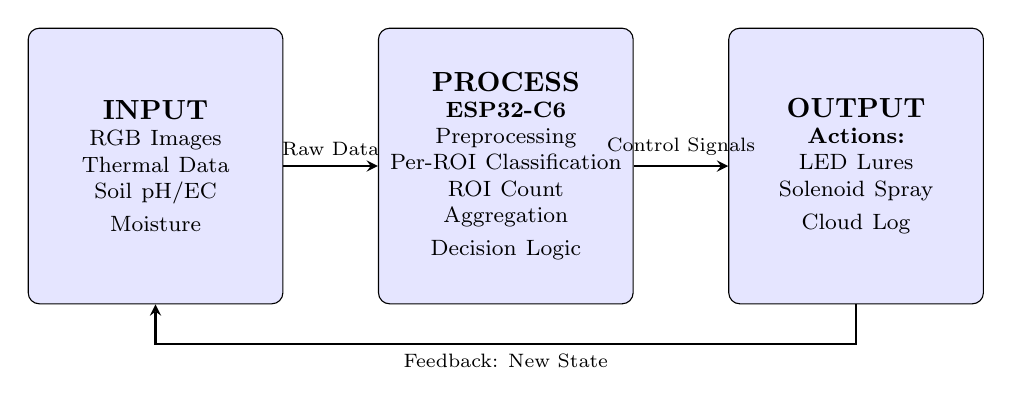
\begin{tikzpicture}[
    node distance=1.2cm,
    auto,
    block/.style={rectangle, draw, fill=blue!10, text width=3cm, align=center, rounded corners, minimum height=3.5cm},
    arrow/.style={thick,->,>=stealth}
]
\node [block] (input) {\textbf{INPUT}\\ \footnotesize RGB Images\\Thermal Data\\Soil pH/EC\\Moisture};
\node [block, right=of input] (process) {\textbf{PROCESS}\\ \footnotesize \textbf{ESP32-C6}\\Preprocessing\\Per-ROI Classification\\ROI Count Aggregation\\Decision Logic};
\node [block, right=of process] (output) {\textbf{OUTPUT}\\ \footnotesize \textbf{Actions:}\\LED Lures\\Solenoid Spray\\Cloud Log};

\draw [arrow] (input) -- node[midway, above, font=\scriptsize] {Raw Data} (process);
\draw [arrow] (process) -- node[midway, above, font=\scriptsize] {Control Signals} (output);
\draw [arrow] (output.south) -- ++(0,-0.5) -| node[pos=0.25, below, font=\scriptsize] {Feedback: New State} (input.south);
\end{tikzpicture}
}
\caption{Conceptual Framework (IPO Model).}
\label{fig:ipo}
\end{figure}

\subsection{Materials and Hardware Robustness}
To withstand Davao's monsoon conditions, the computational unit is housed in an IP65-rated polycarbonate enclosure, providing complete dust ingress protection and resistance to low-pressure water jets per the IEC ingress-protection code \cite{iec60529}. The physical arrangement of these components, including the spatial integration of the directional spray nozzle, the 5MP camera module, the passive pheromone lure, and the soil sensors relative to the target crop, is visualized in the system mockup (Fig.~\ref{fig:mockup}).

\begin{figure}[htbp]
\centering
\includegraphics[width=\columnwidth]{proposal_2_mockup.png}
\caption{Physical mockup of the fixed-post IoT pest monitoring and soil-gated control station, illustrating the spatial integration of hardware components.}
\label{fig:mockup}
\end{figure}

For telemetry, LoRaWAN is utilized over NB-IoT to ensure penetration through dense foliage. Operating on the 915 MHz band with a Spreading Factor (SF) of 10, the system overcomes recognized signal attenuation limits characterized for LoRaWAN links in tropical vegetative canopies \cite{ansah2020}.

The electrical integration is orchestrated by a central Power Management Unit (PMU) detailed in Fig.~\ref{fig:hardware}. The ESP32-C6 handles peripheral communication via SPI for the imaging module and discrete GPIO controls via relays for the 12V solenoid actuator. The economic viability of the node is maintained under a strict budget, consistent with low-cost LoRaWAN agricultural nodes reporting material costs an order of magnitude below commercial stations \cite{viticulture2026}; the itemization is detailed in Table~\ref{tab:bom}.

\begin{figure}[htbp]
\centering
\resizebox{\columnwidth}{!}{%
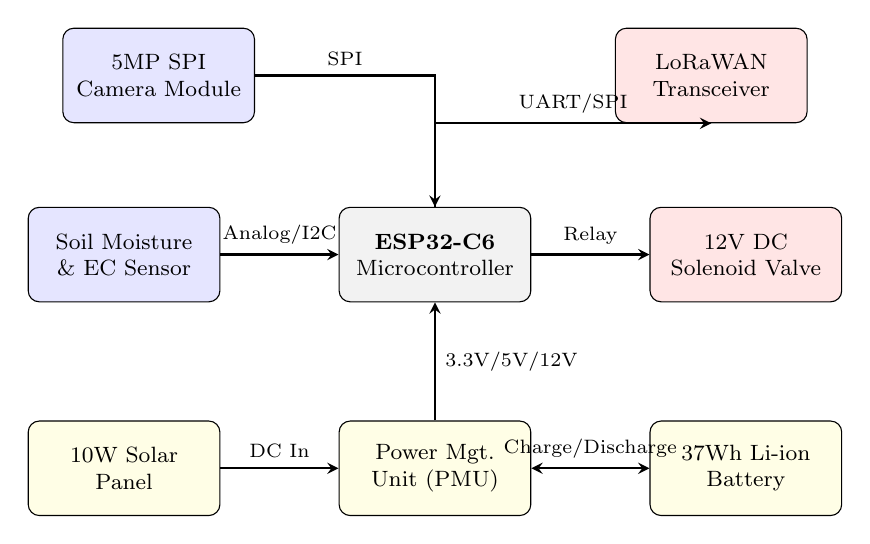
\begin{tikzpicture}[
    node distance=1.5cm,
    auto,
    box/.style={rectangle, draw=black, fill=gray!10, text width=2.2cm, align=center, rounded corners, minimum height=1.2cm, font=\footnotesize},
    sensor/.style={rectangle, draw=black, fill=blue!10, text width=2.2cm, align=center, rounded corners, minimum height=1.2cm, font=\footnotesize},
    actuator/.style={rectangle, draw=black, fill=red!10, text width=2.2cm, align=center, rounded corners, minimum height=1.2cm, font=\footnotesize},
    power/.style={rectangle, draw=black, fill=yellow!10, text width=2.2cm, align=center, rounded corners, minimum height=1.2cm, font=\footnotesize},
    arrow/.style={thick,->,>=stealth}
]
% Nodes
\node [box] (mcu) {\textbf{ESP32-C6}\\Microcontroller};
\node [sensor, above left=of mcu] (cam) {5MP SPI\\Camera Module};
\node [sensor, left=of mcu] (soil) {Soil Moisture\\ \& EC Sensor};
\node [actuator, right=of mcu] (solenoid) {12V DC\\Solenoid Valve};
\node [actuator, above right=of mcu] (lora) {LoRaWAN\\Transceiver};
\node [power, below=of mcu] (pmu) {Power Mgt.\\Unit (PMU)};
\node [power, left=of pmu] (solar) {10W Solar\\Panel};
\node [power, right=of pmu] (batt) {37Wh Li-ion\\Battery};

% Connections
\draw [arrow] (cam) -| node[pos=0.25, above, font=\scriptsize] {SPI} (mcu.north);
\draw [arrow] (soil) -- node[above, font=\scriptsize] {Analog/I2C} (mcu);
\draw [arrow] (mcu) -- node[above, font=\scriptsize] {Relay} (solenoid);
\draw [arrow] (mcu) |- node[pos=0.75, above, font=\scriptsize] {UART/SPI} (lora.south);
\draw [arrow] (solar) -- node[above, font=\scriptsize] {DC In} (pmu);
\draw [thick,<->,>=stealth] (pmu) -- node[above, font=\scriptsize] {Charge/Discharge} (batt);
\draw [arrow] (pmu) -- node[right, font=\scriptsize] {3.3V/5V/12V} (mcu);
\end{tikzpicture}
}
\caption{Hardware Architecture Block Diagram illustrating sensor interfaces, physical actuators, and power distribution.}
\label{fig:hardware}
\end{figure}

\begin{table}[htbp]
\caption{Estimated Bill of Materials (BoM) per Node}
\label{tab:bom}
\centering
\resizebox{0.95\columnwidth}{!}{%
\begin{tabular}{llrr}
\toprule
\textbf{Component Category} & \textbf{Specification} & \textbf{Qty} & \textbf{Est. Cost (PHP)} \\
\midrule
Microcontroller & ESP32-C6 Dev Board & 1 & 450.00 \\
Camera Module & OV5640 5MP (SPI) & 1 & 650.00 \\
Telemetry & LoRaWAN Node (915 MHz) & 1 & 850.00 \\
Sensors & Capacitive Soil Moisture/EC & 1 & 900.00 \\
Actuator & 12V DC Solenoid Valve & 1 & 350.00 \\
Power Supply & 10W Solar Panel + PMU & 1 & 1,200.00 \\
Energy Storage & 10,000 mAh Li-ion Pack & 1 & 800.00 \\
Enclosure & IP65 Polycarbonate Box & 1 & 400.00 \\
Miscellaneous & Relays, PCBs, Pheromones & 1 & 1,000.00 \\
\midrule
\textbf{Total Estimated Cost} & & & \textbf{6,600.00} \\
\bottomrule
\end{tabular}
}
\end{table}

\subsection{Sampling and Sample Size}
A stratified sampling approach is adopted, with the three target species (\textit{T. hawaiiensis}, \textit{E. thrax}, \textit{P. nigronervosa}) forming the strata. For model development, the fine-tuning dataset comprises 150--300 images per class \cite{hayajneh2023}, of which 20\% explicitly models a negative class (water droplets, shadows, dirt, and non-target insects) to ensure construct validity; the dataset is partitioned 70/15/15 into training, validation, and held-out test sets. For the Phase 1 bench validation, specimens are staged at five known density levels ($n = 0, 3, 5, 8, 12$ instances/frame, bracketing $N_{EIL} \approx 5$), with 20 independent trials per level (100 trials total). For the Phase 2 potted-plant test, three Cavendish tissue-cultured seedlings (4--6 leaf stage) are each subjected to 15 actuation runs across three simulated soil-moisture states (dry, intermediate, saturated), yielding 135 actuation observations. The per-condition replicate count was set via an a priori TOST power analysis: assuming a residual standard deviation of $\sigma \approx 1.2$ instances/frame from pilot observations, 20 trials per density level yield $\geq 0.80$ power to declare equivalence within the $\delta = \pm 1$ margin at $\alpha = 0.05$; the same target power motivates the 15 runs per seedling$\times$moisture-state cell. % REVIEW: recompute sigma and n once pilot data exist (e.g., TOSTER/pwr in R).

\subsection{Instruments, Validity, and Reliability}
The research instruments comprise the 5MP RGB camera, the capacitive soil moisture/EC sensor, and a manually operated mechanical counter serving as the ground-truth reference standard. Prior to data collection, the soil moisture/EC sensor is calibrated against gravimetric water-content measurements across the three moisture states, and the camera focal length and lighting are fixed and verified on a calibration target. Instrument reliability is assessed via test--retest repeatability (10 repeated readings per state) and reported as the coefficient of variation. Construct validity of the CNN is reinforced by the negative-class design, and measurement validity of counts is established through the equivalence testing against the mechanical reference.

\subsection{Methods and Procedures: Validation and Logic}
To optimize processing on edge hardware, this study employs transfer learning. Fine-tuning a pre-trained MobileNetV2 backbone requires 150-300 images per class to achieve competitive accuracy \cite{hayajneh2023}. Computational waste is avoided by applying frame-differencing algorithms to crop moving Regions of Interest before classification \cite{prasetyo2022,chaudhari2023}, safely satisfying the inference limits of the ESP32 \cite{donskoy2025}. The system performs per-ROI presence classification on the frame-differenced regions; qualifying ROIs are then counted and aggregated over the 30-minute window to produce $\hat{N}_{pest}$. It is therefore a classify-then-count pipeline rather than a direct density-regression model.

The three-stage control logic ensures chemical intervention is applied accurately. Stage 1 utilizes generic sticky traps baited with aggregation pheromones \cite{klassen2023} to passively lure pests into the focal plane. Stage 2 executes the CNN evaluation. Stage 3 triggers precision spraying, which is electronically aborted if the soil moisture sensor detects ground saturation. The logic dynamically aggregates classifications over a 30-minute window ($\hat{N}_{pest}$):
\begin{equation}
\text{Action} =
\begin{cases}
\text{Spray}, & \text{if } \hat{N}_{pest} > N_{EIL} \land \text{Soil}_{\text{safe}} = 1 \\
\text{Log}, & \text{otherwise}
\end{cases}
\end{equation}

\subsection{Statistical Analysis}
All inferential tests are conducted at a significance level of $\alpha = 0.05$. CNN performance is reported using Precision, Recall, and $F1$-score, with the $\geq 85\%$ criterion applied to the mean held-out $F1$-score. Detection equivalence between prototype and ground-truth counts is assessed using a Two One-Sided Tests (TOST) procedure with a pre-registered equivalence margin of $\delta = \pm 1$ instance/frame; equivalence is concluded if the $90\%$ confidence interval of the mean difference lies entirely within $[-\delta, +\delta]$. Actuation reliability is evaluated against the $95\%$ target using an exact binomial proportion test, and battery autonomy against the 7-day threshold using a one-sample test. Outliers in the sensor logs are filtered using the Median Absolute Deviation (MAD):
\begin{equation}
MAD = median(|X_i - \tilde{X}|)
\end{equation}
A $3 \times MAD$ threshold is selected to preserve biological outbreak events while filtering electronic anomalies.

\subsection{Project Milestones and Contingencies}
To guarantee that the project satisfies the strict resource limits and scope boundaries of a standard undergraduate capstone, the validation has been thoroughly divided into two time-bound stages. The specific deliverables, milestones, and contingency protocols are defined in Table~\ref{tab:milestones}.

\begin{table}[htbp]
\caption{Two-Semester Project Milestones and Contingencies}
\label{tab:milestones}
\centering
\resizebox{\columnwidth}{!}{%
\begin{tabular}{llp{4cm}}
\toprule
\textbf{Phase} & \textbf{Primary Task} & \textbf{Success Criteria / Contingency} \\
\midrule
Sem 1 & Trade-off Analysis & Documented comparison of MCUs/Sensors / Default to ESP32-C6. \\
Sem 1 & Hardware/Firmware Integration & Sensors interface properly / Switch to generic dev board if custom PCB fails. \\
Sem 1 & Dataset \& MobileNetV2 Tuning & $\geq 85\%$ F1-Score / Expand dataset by 50 images per class if accuracy fails. \\
Sem 1 & Phase 1 Bench Validation & Successful detection on servo-rig / Adjust lighting/focal length. \\
Sem 2 & Phase 2 Potted Plant Test & Solenoid fires accurately to logic / Recalibrate soil sensor thresholds. \\
Sem 2 & Power Autonomy Verification & $>$7 days sustained battery / Reduce cycle frequency to 45 mins. \\
Sem 2 & Final Documentation & Manuscript ready 1 week prior to defense. \\
\bottomrule
\end{tabular}
}
\end{table}

\begin{thebibliography}{21}

\bibitem{reyes2022} C. P. Reyes \textit{et al.}, ``Molecular Characterization and Assessment of Abundance of \textit{Thrips hawaiiensis} (Morgan, 1913) on Three Plantations of Cavendish Banana in Davao del Norte, Philippines,'' \textit{Philipp. J. Sci.}, vol. 151, no. 3, pp. 1049--1065, 2022. \url{https://doi.org/10.56899/151.03.21}

\bibitem{nozawa2023} S. Nozawa \textit{et al.}, ``\textit{Fusarium mindanaoense} sp. nov., a New Fusarium Wilt Pathogen of Cavendish Banana from the Philippines,'' \textit{J. Fungi}, vol. 9, no. 4, p. 443, 2023. \url{https://doi.org/10.3390/jof9040443}

\bibitem{vercellino2022} R. B. Vercellino \textit{et al.}, ``Agricultural weeds: the contribution of domesticated species to the origin and evolution of feral weeds,'' \textit{Pest Manag. Sci.}, vol. 79, no. 3, pp. 922--934, 2022. \url{https://doi.org/10.1002/ps.7321}

\bibitem{liu2020} X. Liu \textit{et al.}, ``Comparative effects of the recovery from sulfuric and nitric acid rain on the soil enzyme activities and metabolic functions of soil microbial communities,'' \textit{Sci. Total Environ.}, vol. 714, p. 136788, 2020. \url{https://doi.org/10.1016/j.scitotenv.2020.136788}

\bibitem{zeyliger2023} A. Zeyliger \textit{et al.}, ``Assessment of Irrigation Efficiency by Coupling Remote Sensing and Ground-Based Data: Case Study of Sprinkler Irrigation of Alfalfa in the Saratovskoye Zavolgie Region of Russia,'' \textit{Sensors}, vol. 23, no. 5, p. 2601, 2023. \url{https://doi.org/10.3390/s23052601}

\bibitem{ahmed2024} S. Ahmed \textit{et al.}, ``IoT based intelligent pest management system for precision agriculture,'' \textit{Sci. Rep.}, vol. 14, p. 31917, 2024. \url{https://doi.org/10.1038/s41598-024-83012-3}

\bibitem{cardoso2022} B. Cardoso \textit{et al.}, ``Internet of Things Meets Computer Vision to Make an Intelligent Pest Monitoring Network,'' \textit{Appl. Sci.}, vol. 12, no. 18, p. 9397, 2022. \url{https://doi.org/10.3390/app12189397}

\bibitem{deoliveira2025} B. L. de Oliveira \textit{et al.}, ``Fostering a Framework for Secure Data Transfer From IoT Devices To Cloud,'' \textit{Procedia Comput. Sci.}, vol. 263, pp. 418--425, 2025. \url{https://doi.org/10.1016/j.procs.2025.07.051}

\bibitem{bereciartua2023} A. Bereciartua-P\'erez \textit{et al.}, ``Multiclass insect counting through deep learning-based density maps estimation,'' \textit{Smart Agric. Technol.}, vol. 4, p. 100125, 2023. \url{https://doi.org/10.1016/j.atech.2022.100125}

\bibitem{hayajneh2023} A. M. Hayajneh \textit{et al.}, ``Tiny machine learning on the edge: A framework for transfer learning empowered unmanned aerial vehicle assisted smart farming,'' \textit{IET Smart Cities}, vol. 5, no. 1, pp. 1--15, 2023. \url{https://doi.org/10.1049/smc2.12072}

\bibitem{donskoy2025} D. Donskoy \textit{et al.}, ``TinyML Classification for Agriculture Objects with ESP32,'' \textit{Digit.}, vol. 5, no. 4, p. 48, 2025. \url{https://doi.org/10.3390/digital5040048}

\bibitem{singh2022} N. Singh \textit{et al.}, ``Semantic segmentation of in-field cotton bolls from the sky using deep convolutional neural networks,'' \textit{Smart Agric. Technol.}, vol. 3, p. 100045, 2022. \url{https://doi.org/10.1016/j.atech.2022.100045}

\bibitem{prasetyo2022} E. Prasetyo \textit{et al.}, ``Yolov4-tiny with wing convolution layer for detecting fish body part,'' \textit{Comput. Electron. Agric.}, vol. 198, p. 107023, 2022. \url{https://doi.org/10.1016/j.compag.2022.107023}

\bibitem{chaudhari2023} V. Chaudhari and M. P. Patil, ``Detection and Classification of Banana Leaf Disease Using Novel Segmentation and Ensemble Machine Learning Approach,'' \textit{Appl. Comput. Syst.}, vol. 28, no. 1, pp. 92--99, 2023. \url{https://doi.org/10.2478/acss-2023-0009}

\bibitem{wang2024} Z. Wang \textit{et al.}, ``IoT-based system of prevention and control for crop diseases and insect pests,'' \textit{Front. Plant Sci.}, vol. 15, p. 1323074, 2024. \url{https://doi.org/10.3389/fpls.2024.1323074}

\bibitem{sneineh2023} A. Abu Sneineh and A. A. A. Shabaneh, ``Design of a smart hydroponics monitoring system using an ESP32 microcontroller and the Internet of Things,'' \textit{MethodsX}, vol. 11, p. 102401, 2023. \url{https://doi.org/10.1016/j.mex.2023.102401}

\bibitem{demandar2026} E. Demandar-Paraguya and C. P. Campana, ``Transforming Sigatoka Management Through Precision Agriculture: The Role of Drone Spraying in Cavendish Banana in Region XI and XII,'' \textit{Int. J. Res. Publ. Rev.}, vol. 7, no. 1, 2026. [Online]. Available: \url{https://ijrpr.com/uploads/V7ISSUE1/IJRPR58863.pdf}

\bibitem{iec60529} International Electrotechnical Commission, ``Degrees of protection provided by enclosures (IP Code),'' IEC Standard 60529:1989+AMD1:1999+AMD2:2013. [Online]. Available: \url{https://webstore.iec.ch/publication/2452}

\bibitem{ansah2020} R. Ansah \textit{et al.}, ``Characterising foliage influence on LoRaWAN pathloss in a tropical vegetative environment,'' \textit{IET Wireless Sensor Systems}, vol. 10, no. 5, 2020. \url{https://doi.org/10.1049/iet-wss.2019.0201} % REVIEW: confirm exact page range.

\bibitem{viticulture2026} ``A Versatile and Low-Cost IoT Solution for Bioclimatic Monitoring in Precision Viticulture,'' \textit{Future Internet}, vol. 18, no. 1, art. 16, 2026. \url{https://doi.org/10.3390/fi18010016} % REVIEW: confirm author list from DOI.

\bibitem{klassen2023} D. Klassen, M. D. Lennox, M.-J. Dumont, G. Chouinard, and J. R. Tavares, ``Dispensers for pheromonal pest control,'' \textit{J. Environ. Manage.}, vol. 325, p. 116590, 2023. \url{https://doi.org/10.1016/j.jenvman.2022.116590}

\end{thebibliography}

\end{document}
